% Options for packages loaded elsewhere
\PassOptionsToPackage{unicode}{hyperref}
\PassOptionsToPackage{hyphens}{url}
\PassOptionsToPackage{dvipsnames,svgnames,x11names}{xcolor}
%
\documentclass[
  letterpaper,
  DIV=11,
  numbers=noendperiod]{scrreprt}

\usepackage{amsmath,amssymb}
\usepackage{lmodern}
\usepackage{iftex}
\ifPDFTeX
  \usepackage[T1]{fontenc}
  \usepackage[utf8]{inputenc}
  \usepackage{textcomp} % provide euro and other symbols
\else % if luatex or xetex
  \usepackage{unicode-math}
  \defaultfontfeatures{Scale=MatchLowercase}
  \defaultfontfeatures[\rmfamily]{Ligatures=TeX,Scale=1}
\fi
% Use upquote if available, for straight quotes in verbatim environments
\IfFileExists{upquote.sty}{\usepackage{upquote}}{}
\IfFileExists{microtype.sty}{% use microtype if available
  \usepackage[]{microtype}
  \UseMicrotypeSet[protrusion]{basicmath} % disable protrusion for tt fonts
}{}
\makeatletter
\@ifundefined{KOMAClassName}{% if non-KOMA class
  \IfFileExists{parskip.sty}{%
    \usepackage{parskip}
  }{% else
    \setlength{\parindent}{0pt}
    \setlength{\parskip}{6pt plus 2pt minus 1pt}}
}{% if KOMA class
  \KOMAoptions{parskip=half}}
\makeatother
\usepackage{xcolor}
\setlength{\emergencystretch}{3em} % prevent overfull lines
\setcounter{secnumdepth}{-\maxdimen} % remove section numbering
% Make \paragraph and \subparagraph free-standing
\ifx\paragraph\undefined\else
  \let\oldparagraph\paragraph
  \renewcommand{\paragraph}[1]{\oldparagraph{#1}\mbox{}}
\fi
\ifx\subparagraph\undefined\else
  \let\oldsubparagraph\subparagraph
  \renewcommand{\subparagraph}[1]{\oldsubparagraph{#1}\mbox{}}
\fi


\providecommand{\tightlist}{%
  \setlength{\itemsep}{0pt}\setlength{\parskip}{0pt}}\usepackage{longtable,booktabs,array}
\usepackage{calc} % for calculating minipage widths
% Correct order of tables after \paragraph or \subparagraph
\usepackage{etoolbox}
\makeatletter
\patchcmd\longtable{\par}{\if@noskipsec\mbox{}\fi\par}{}{}
\makeatother
% Allow footnotes in longtable head/foot
\IfFileExists{footnotehyper.sty}{\usepackage{footnotehyper}}{\usepackage{footnote}}
\makesavenoteenv{longtable}
\usepackage{graphicx}
\makeatletter
\def\maxwidth{\ifdim\Gin@nat@width>\linewidth\linewidth\else\Gin@nat@width\fi}
\def\maxheight{\ifdim\Gin@nat@height>\textheight\textheight\else\Gin@nat@height\fi}
\makeatother
% Scale images if necessary, so that they will not overflow the page
% margins by default, and it is still possible to overwrite the defaults
% using explicit options in \includegraphics[width, height, ...]{}
\setkeys{Gin}{width=\maxwidth,height=\maxheight,keepaspectratio}
% Set default figure placement to htbp
\makeatletter
\def\fps@figure{htbp}
\makeatother
\newlength{\cslhangindent}
\setlength{\cslhangindent}{1.5em}
\newlength{\csllabelwidth}
\setlength{\csllabelwidth}{3em}
\newlength{\cslentryspacingunit} % times entry-spacing
\setlength{\cslentryspacingunit}{\parskip}
\newenvironment{CSLReferences}[2] % #1 hanging-ident, #2 entry spacing
 {% don't indent paragraphs
  \setlength{\parindent}{0pt}
  % turn on hanging indent if param 1 is 1
  \ifodd #1
  \let\oldpar\par
  \def\par{\hangindent=\cslhangindent\oldpar}
  \fi
  % set entry spacing
  \setlength{\parskip}{#2\cslentryspacingunit}
 }%
 {}
\usepackage{calc}
\newcommand{\CSLBlock}[1]{#1\hfill\break}
\newcommand{\CSLLeftMargin}[1]{\parbox[t]{\csllabelwidth}{#1}}
\newcommand{\CSLRightInline}[1]{\parbox[t]{\linewidth - \csllabelwidth}{#1}\break}
\newcommand{\CSLIndent}[1]{\hspace{\cslhangindent}#1}

\KOMAoption{captions}{tableheading}
\makeatletter
\makeatother
\makeatletter
\makeatother
\makeatletter
\@ifpackageloaded{caption}{}{\usepackage{caption}}
\AtBeginDocument{%
\ifdefined\contentsname
  \renewcommand*\contentsname{Table of contents}
\else
  \newcommand\contentsname{Table of contents}
\fi
\ifdefined\listfigurename
  \renewcommand*\listfigurename{List of Figures}
\else
  \newcommand\listfigurename{List of Figures}
\fi
\ifdefined\listtablename
  \renewcommand*\listtablename{List of Tables}
\else
  \newcommand\listtablename{List of Tables}
\fi
\ifdefined\figurename
  \renewcommand*\figurename{Figure}
\else
  \newcommand\figurename{Figure}
\fi
\ifdefined\tablename
  \renewcommand*\tablename{Table}
\else
  \newcommand\tablename{Table}
\fi
}
\@ifpackageloaded{float}{}{\usepackage{float}}
\floatstyle{ruled}
\@ifundefined{c@chapter}{\newfloat{codelisting}{h}{lop}}{\newfloat{codelisting}{h}{lop}[chapter]}
\floatname{codelisting}{Listing}
\newcommand*\listoflistings{\listof{codelisting}{List of Listings}}
\makeatother
\makeatletter
\@ifpackageloaded{caption}{}{\usepackage{caption}}
\@ifpackageloaded{subcaption}{}{\usepackage{subcaption}}
\makeatother
\makeatletter
\@ifpackageloaded{tcolorbox}{}{\usepackage[many]{tcolorbox}}
\makeatother
\makeatletter
\@ifundefined{shadecolor}{\definecolor{shadecolor}{rgb}{.97, .97, .97}}
\makeatother
\makeatletter
\makeatother
\ifLuaTeX
  \usepackage{selnolig}  % disable illegal ligatures
\fi
\IfFileExists{bookmark.sty}{\usepackage{bookmark}}{\usepackage{hyperref}}
\IfFileExists{xurl.sty}{\usepackage{xurl}}{} % add URL line breaks if available
\urlstyle{same} % disable monospaced font for URLs
\hypersetup{
  colorlinks=true,
  linkcolor={blue},
  filecolor={Maroon},
  citecolor={Blue},
  urlcolor={Blue},
  pdfcreator={LaTeX via pandoc}}

\author{}
\date{}

\begin{document}
\ifdefined\Shaded\renewenvironment{Shaded}{\begin{tcolorbox}[frame hidden, borderline west={3pt}{0pt}{shadecolor}, enhanced, breakable, interior hidden, boxrule=0pt, sharp corners]}{\end{tcolorbox}}\fi

\hypertarget{week-1}{%
\chapter{Week 1}\label{week-1}}

\hypertarget{summary}{%
\section{Summary}\label{summary}}

Among the many points addressed in the lecture were: 1. Earth
Observation data uses electromagnetic radiation reflected or emitted
from the object or area of interest that travels at the speed of light
(because electromagnetic radiation is light itself!?!?). and 2. Some
objects, or rather, electromagnetic radiation in a certain spectrum
which cannot be viewed by human eyes can be detected by satellite
sensors to allow human eyes to see them. Because colours are nothing but
light, and light is nothing but electromagnetic radiation and
electromagnetic radiation consists of different waves which is part of
the electromagnetic spectrum ?!?! And human eyes can only see only a
small range within the electromagnetic radiation spectrum! (this blows
my mind as I write. Am I supposed to have known this as someone who
finished primary education a number of years ago?)

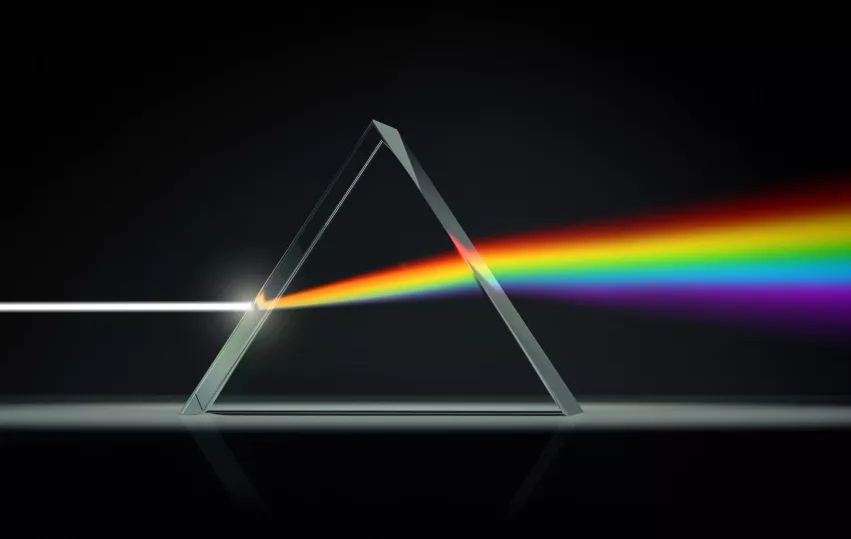
\includegraphics{light electromagnetic radiation.png}

Take leaves or vegetation as an example. They can be viewed in the
visible spectrum but also in the near-infrared light.

Firstly, why leaves green? Wavelengths in the green region of the
electromagnetic spectrum are reflected by pigments in the leaf' (NASA
Science). That's why we see green leaves. But also `a plant with more
chlorophyll (pigment) will reflect more near-infrared energy than an
unhealthy plant' (NASA Science). So this is why with satellite imagery,
we can use both the visible and invisible near-infrared spectrum to
study vegetation.

SCATTERING: Why is the sky black on the moon? (no atmosphere) Why is the
sky blue? (short waves scattered) Why is the sky red when the sun goes
down?

Why is the ocean blue? - water absorbs the red yellow and green waves
but reflects /scatters blue.

Finally, there are two types of sensors to record electromagnetic
radiation.

1. Passive sensors record EMR reflected or emitted from the terrain.

2. Active sensors such as LiDAR (on aircrafts), SAR or RADAR emit
electromagnetic waves and record the amount of radiant flux (energy per
unit of time) that travelled back to the sensors. These are used to
develop the DEM, digital elevation model, using the speed of travel to
measure the distance between the point on the terrain and the location
of the sensor. SAR can see through clouds.

\hypertarget{application}{%
\section{Application}\label{application}}

\begin{enumerate}
\def\labelenumi{\arabic{enumi}.}
\item
  What drew me to Earth Observation data in the first place is my
  frustration due the lack of granularity of urban/rural classifications
  in population-based health surveys. There is usually only two groups
  of residence: urban or rural. But when I got to know that satellite
  imagery may be used to classify urban settlements into formal and
  informal settlements, I got interested in exploring this further.
  Different characteristics of informal settlements can be used in
  combination of ML classification tasks. (Kuffer, Pfeffer, and Sliuzas
  2016)
\item
  In the field of global public health, malaria or infectious disease
  epidemiologists have been the forerunner in using geospatial data
  including Earth Observation data. For example, this paper by Brousse
  et al. (2020) uses the urban classification data, based on the Local
  Climate Zone map which is developed based on satellite imagery, to
  predict malaria prevalence.
\item
  Surface temperature

  `Heat' is such a big topic these days. Many climate \& health research
  investigates the effect of `heat' on health. How can we get land
  surface temperature data? I read that Land Surface Temperature is
  derived from thermal infrared data, which is in the wavelength range
  of 0.75 -15 μm. This particular wavelength range can be recorded by a
  multispectoral scanner on Landsat 8, MODIS, ASTER etc etc.
\end{enumerate}

\hypertarget{reflection}{%
\section{Reflection}\label{reflection}}

It has taken me some time to absorb this week's concept. What has helped
me understand is the fact that there is no such thing as colour,
``colours do not exist, what exist is light''. Different objects reflect
or absorb light in different ways (eg as I explained of green leaves)
and satellite sensors and earth observation data take advantage of this
fact.

\hypertarget{refs}{}
\begin{CSLReferences}{1}{0}
\leavevmode\vadjust pre{\hypertarget{ref-Brousse2020}{}}%
Brousse, O, S Georganos, M Demuzere, S Dujardin, M Lennert, C Linard, R
W Snow, W Thiery, and N P M van Lipzig. 2020. {``Can We Use Local
Climate Zones for Predicting Malaria Prevalence Across Sub-Saharan
African Cities?''} \emph{Environmental Research Letters} 15 (12):
124051. \url{https://doi.org/10.1088/1748-9326/abc996}.

\leavevmode\vadjust pre{\hypertarget{ref-kuffer2016}{}}%
Kuffer, Monika, Karin Pfeffer, and Richard Sliuzas. 2016. {``Slums from
Space{\textemdash}15 Years of Slum Mapping Using Remote Sensing.''}
\emph{Remote Sensing} 8 (6): 455.
\url{https://doi.org/10.3390/rs8060455}.

\end{CSLReferences}



\end{document}
